% Architecture planning | How the application was planned to implement

\section{Methodology}

The human-presentator project was initially conceived as a streamlined, single-script Python
application designed to generate talking-head animations from static images and text input. The
original approach emphasized simplicity and cohesion, with all functionality consolidated into one
comprehensive Python script that would handle the entire pipeline from text input to final video
output.

Rather than developing proprietary solutions from scratch, the project methodology centered on
leveraging established open-source software for the core voice generation and image animation
components. This approach was chosen to reduce development time by building upon proven, well-tested
codebases, ensure compatibility with existing workflows and standards and maintain transparency and
auditability through open-source implementations.

An integral component of the original methodology included implementing automated validation
mechanisms for the generated MP4 output files. The automated validation approach aimed to ensure
consistent output quality while reducing manual review overhead during the development and testing
phases.

The initial architectural approach emphasized a monolithic design pattern, consolidating all
processing stages within a single executable unit. This methodology was selected to minimize
deployment complexity, reduce inter-component communication overhead, and provide a clear, linear
processing flow that could be easily understood and modified by developers working on the project.

\subsection{Usage Recipe}

% How to use the application

\textbf{Usecase}: Generate a talking-Presenter animation from a static image, text and audio input.
\textbf{Prequisites}: Linux, Docker, NVIDIA GPU with CUDA support (recommended for performance).
\textbf{Time}: Approximately 10 minutes for setup and 5min-24h in execution.


\begin{enumerate}
    \item Clone Repository \mintinline{bash}{git clone https://github.com/Squad-Mandalore/human-presentator.git}
    \item Change directory to the project root: \mintinline{bash}{cd human-presentator}
    \item Build the Application: \mintinline{bash}{docker compose up}
    \item Open the User-Interface in your browser: \mintinline{bash}{http://localhost:8000}
\end{enumerate}

\begin{figure}[H]
  \centering
  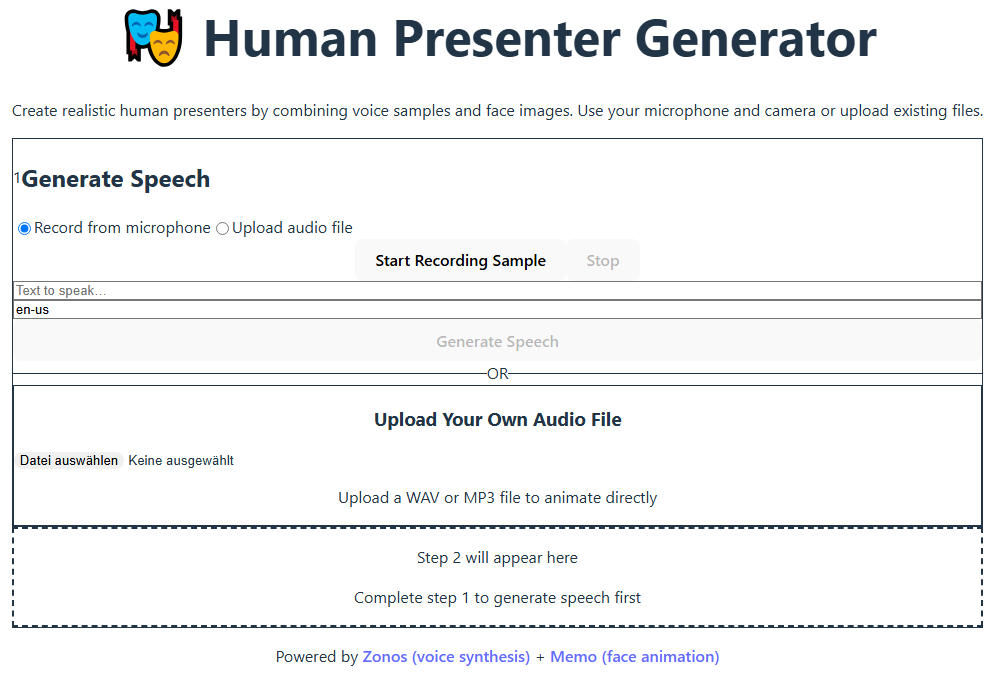
\includegraphics[width=\textwidth, keepaspectratio]{ui-picture.png}
  \caption{User Interface of the Human Presentor}
  \label{fig:architecture}
\end{figure}

\begin{enumerate}
    \item Prepare your data:
    \item (optional) Step 1: Generate Audio
        \begin{itemize}
            \item Select Record from microphone or Upload Audio File
            \item Insert the text you want the speaker to say.
            \item Select \texttt{Generate Speech}
            \item Wait for the audio file to be generated.
        \end{itemize}
    \item Step 2: Generate Lip-Sync
        \begin{itemize}
            \item Upload Generated Audio File or any pre-recorded audio file.
            \item Upload a static image or use Capture Face Snapshot for a presentor image.
            \item Select \texttt{Generate Video}
            \item Wait for the video to be generated.
        \end{itemize}
\end{enumerate}

\subsection{Development Recipe}

How to use the application components for own development or research purposes. The Structure of the human-presentator is defined into multiple directories, each containing a specific component of the application. 
This Recipe can also be used to rebuild the human-presentator project from scratch. 
\textbf{Usecase}: Develop or extend the human-presentator project for research or production purposes.
\textbf{Prequisites}: Linux, Python, NodeJS, Docker, NVIDIA GPU with CUDA support (optional but recommended for performance), Python.
\textbf{Time}: Unkown, depends on the development task.
The main components are:
\begin{itemize}
    \item \texttt{zonos-api}: Voice cloning and text-to-speech components, utilizing \gls{Zonos}.
    \item \texttt{memo-api}: Lip-sync and animation components, utilizing \gls{memo}.
    \item \texttt{presentator}: Development Script for experimenting with zonos- and memo-api.
    \item \texttt{presentor-vue}: Web user interface for interacting with the zonos- and memo-api.
    \item \texttt{presentation}: Presentation of the human-presentator project.
    \item \texttt{documentation}: Documentation of the human-presentator including this cookbook.
\end{itemize}

\textbf{zonos-api}: The zonos-controller is used as endpoint for utilizing zonos-service for voice cloning and text-to-speech components. 
The zonos-service is responsible for handling the voice cloning and text-to-speech requests, processing the audio / text input, and returning the generated audio output. 
For this purpose \gls{Zonos} have been forked and installed as dependency to implement into the zonos-service.
\textbf{memo-api}: The memo-controller is used as endpoint for utilizing memo-service for lip-sync and animation components.
The memo-service is responsible for handling the lip-sync and animation requests, processing the audio / image input, and returning the generated video output.
For this purpose \gls{memo} have been forked and installed as dependency to implement into the memo-service.

\textbf{presentor-vue}: Contains the Vue.js frontend application that provides a user interface for interacting with the zonos-api and memo-api services.
The frontend allows users to upload audio files, static images, and text input, and displays the generated video output.